\section{Experiment}\label{exp}
We integrated the three most common force of infection models, \case{1a}, \case{1b}, and \case{2b},
plus the proposed model, denoted \case{4*},
into an existing model of heterosexual HIV transmission in Eswatini \cite{TBD}.
 Models \case{2a} and \case{3} were omitted
 as we could not find any example of their use in the literature.
Full details of the transmission model are given in \cite{TBD},
and key details are given in Appendix~\ref{esw}.
% JK: can cut this down if needed...
Briefly, the model includes:
five stages of HIV infection, stratified by acute infection and CD4 count;
five states of connection to treatment;
two sexes and four risk strata, including
higher and lower risk female sex workers (FSW) and their clients.
Risk groups have different numbers and mixing of partners, prevalence of STI symptoms,
and rates of testing, treatment initiation, and treatment failure/discontinuation.
Four types of partnership are modelled, with different
durations, sex frequency, and levels of anal sex and condom use.
\par
Using the Eswatini HIV transmission model, 
we examined the influence of each force of infection model on the:
1)~epidemic dynamics with equal parameters;
2)~modelled proportion of transmission attributed to
different risk groups and/or partnership types throughout the epidemic; and
3)~transmission population attributable fraction \cite{Mishra2014}
of different risk groups and partnership types.
\subsection{Equal Parameters}\label{exp.ep}
First, to explore fundamental differences in epidemic dynamics under each model,
we simulated the Eswatini HIV epidemic under each model with identical parameter values.
Parameter values were taken from
the top 1000 of 100,000 model \case{4*} fits (highest likelihood).
Since models \case{1-2} use the $QA$ parameterization, not $CF$, we defined
$Q_{ijk} = C_{ijk} / \delta_k$, $A_{k} = F_{k} \delta_k$ for \case{1a}, and
$Q_{ijk} = C_{ijk}$, $A_{k} = F_{k}$ for \case{1b} and \case{2b}.
Figure~\ref{fig:ep.inc} illustrates HIV incidence under each model,
stratified by: FSW, their clients, and everyone else (``wider population'');
Figure~\ref{fig:ep.prev} illustrates prevalence.
\begin{figure}[h]
  \centerline{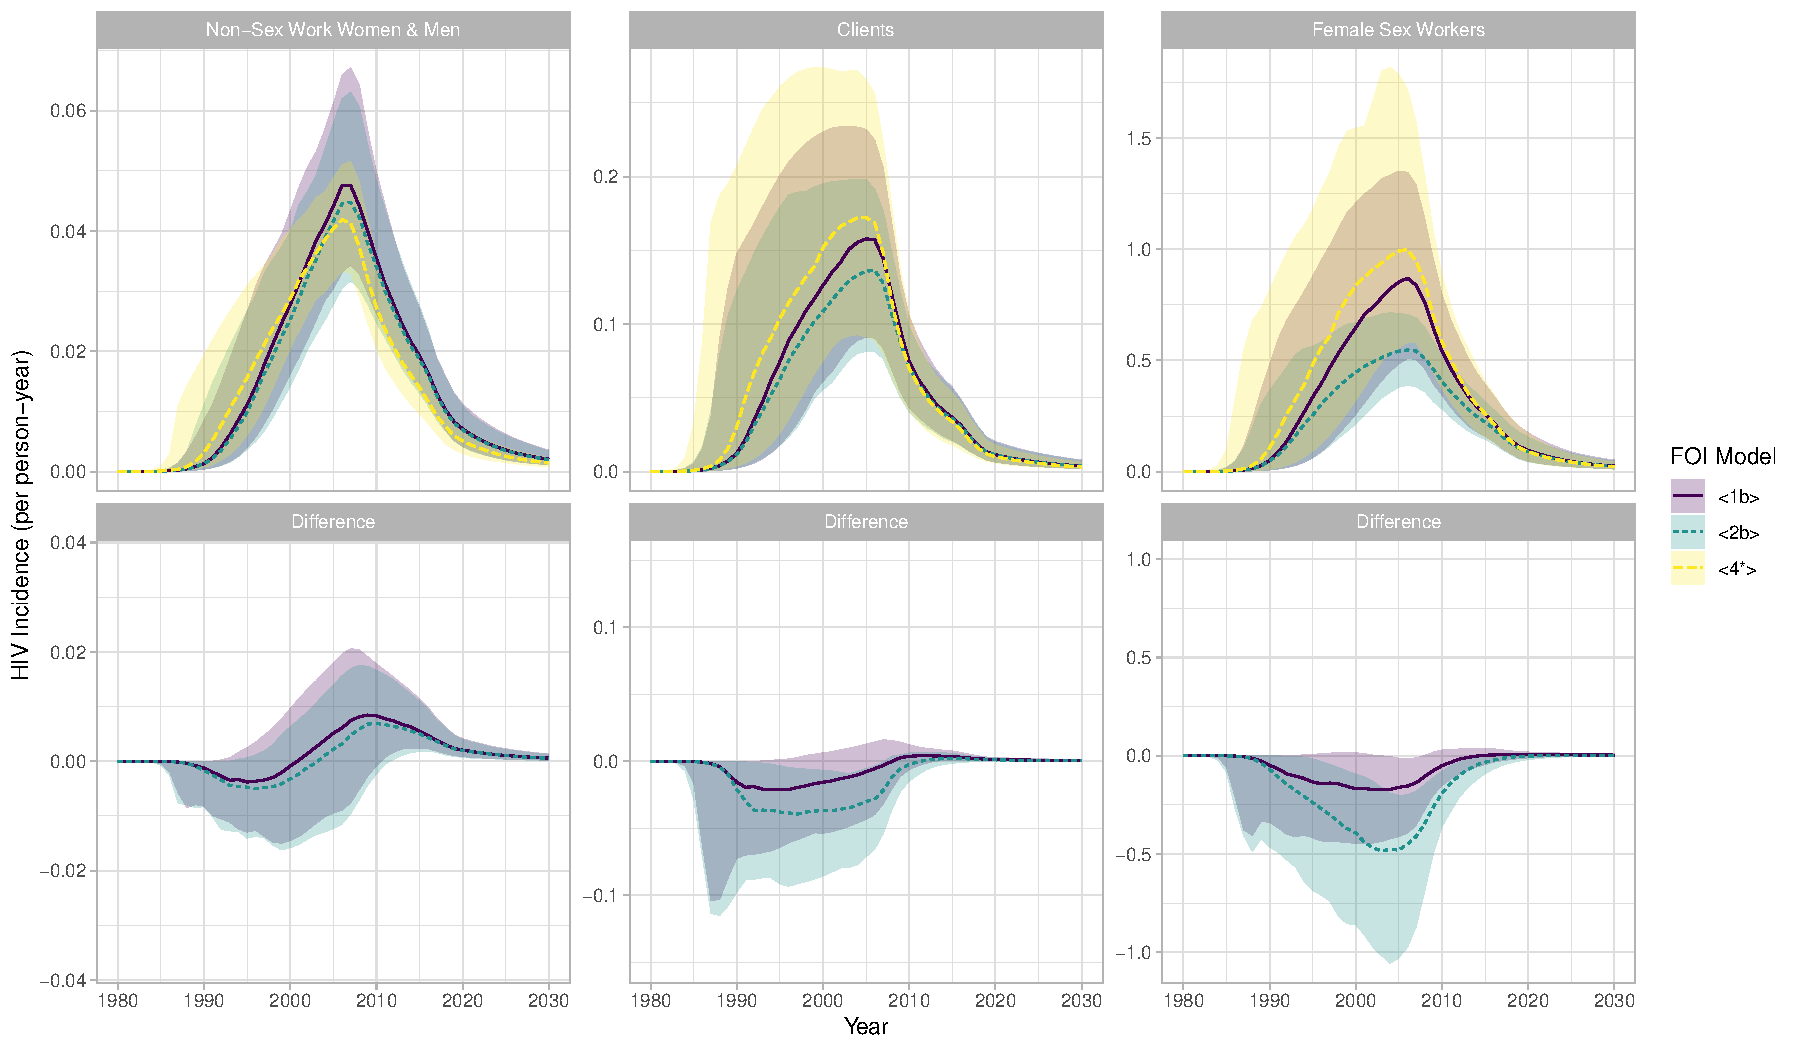
\includegraphics[width=\widefig]{foi.ep.incidence}}
  \caption{Comparison of modelled incidence under force of infection models
    \case{1a}, \case{1b}, \case{2b}, and \case{4*} with equal parameters}
  \label{fig:ep.inc}
  \floatfoot
  FOI Model names:
  \case{1a} binomial per-partnership;
  \case{1b} binomial per-partnership-year;
  \case{2b} binomial per-year;
  \case{4*} partnership exclusion (proposed).
  Parameter values taken from the \case{4*} model fit with highest likelihood;
  for \case{1a}: $Q_{ijk} = C_{ijk} / \delta_k$, $A_{k} = F_{k} \delta_k$;
  for \case{1b} and \case{2b}: $Q_{ijk} = C_{ijk}$, $A_{k} = F_{k}$.
  Lines show median values and transparent ribbons show 90\% confidence intervals
  from top 1000 of 100,000 \case{4*} model fits.
\end{figure}
\par
In the early epidemic, model \case{4*} (yellow) consistently yielded higher incidence
vs models \case{1b} (blue) and \case{2b} (green),
because incidence in \case{4*} is linear before any seroconcordant HIV+ partnerships emerge
--- i.e. while states $\k > 0$ are empty.
By contrast, models \case{1a}, \case{1b}, and \case{2b} all reduce incidence from the outset
as an adjustment for repeated contacts, some of which effectively reflect \emph{future} contacts.
Early incidence under \case{1a} (purple) was also greater than \case{1b} and \case{2b},
which may seem counterintuitive because \case{1a} uses $A = F \delta$ and $Q = C / \delta$,
reducing transmission via longer duration partnerships.
However, for shorter duration partnerships ($\delta < 1$) that dominate early transmission,
model \case{1a} results in more partnerships ($Q > C$) with fewer contacts ($A < F$),
and thus less influence of the binomial adjustment as compared to models \case{1b} and \case{2b}.
Early incidence was similar under models \case{4*} and \case{1a},
but higher in \case{1a} under conditions (model fits) where
regular sex work partnership durations were shorter and
individual clients bought less sex (results not shown).
Such conditions result in less binomial adjustment for sex work partnerships in \case{1a},
and faster ``saturation'' of partnerships among client in \case{4*}.
Finally, \case{2b} yielded the lowest incidence of all,
due to the application of the binomial adjustment to all yearly contacts per-person,
rather than just per-partnership as in \case{1a} and \case{1b}.
\par
% TODO: mid/late epidemic
\clearpage
\subsection{Distribution of Infections}\label{exp.inf}
% JK: honestly, this section feels repetitive with / similar to {exp.tpaf}
%     I would be open to dropping (into appendix) one of the two sections
Next, to explore differences in transmission networks under each model,
we computed the distributions of yearly infections
after calibrating each model to the same targets.
As before, the top 1000 of 100,000 model fits were used in each case.
Figure~\ref{fig:inf.part} illustrates the proportions of yearly infections
transmitted via each partnership type under each calibrated model;
Figure~\ref{fig:inf.from} stratifies by the transmitting risk group,
Figure~\ref{fig:inf.from} by the acquiring group, and
Figure~\ref{fig:inf.alluvial} by all three factors (model \case{4*} only).
\begin{figure}[h]
  \centerline{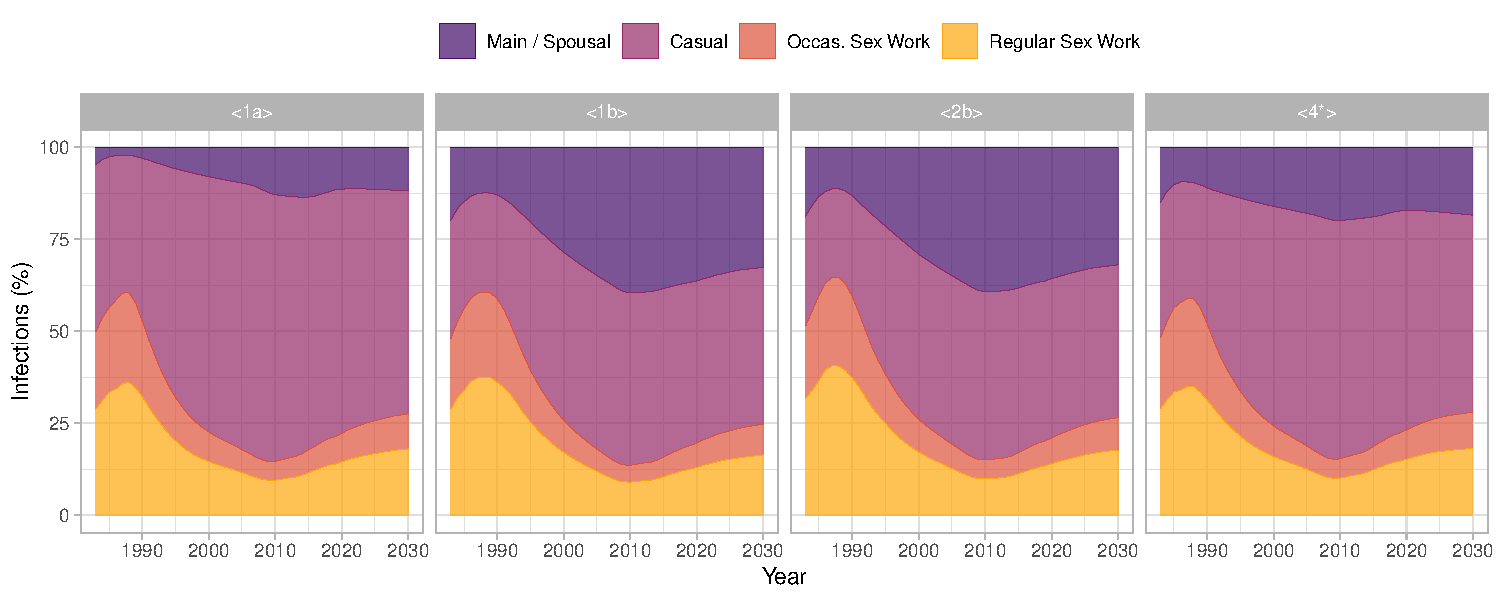
\includegraphics[width=\widefig]{inf-foi-part-rel}}
  \caption{Comparison of the distribution of yearly infections by partnership type
    under calibrated force of infection models \case{1a}, \case{1b}, \case{2b}, and \case{4*}}
  \label{fig:inf.part}
  \floatfoot
  FOI Model names:
  \case{1a} binomial per-partnership;
  \case{1b} binomial per-partnership-year;
  \case{2b} binomial per-year;
  \case{4*} partnership exclusion (proposed).
  Parameters were re-calibrated for each FOI model,
  and infections reflect the median value from
  the top 1000 of 100,000 model fits in each case.
\end{figure}
\par
After calibration, the proportions of infections transmitted
via occasional and regular sex work partnerships were roughly consistent across models
(Figure~\ref{fig:inf.part}).
Conversely, we found large differences between models in yearly infections transmitted
via main/spousal vs casual partnerships.
Specifically, main/spousal partnerships
never contributed more than 15\% of infections under \case{1a} or 20\% under \case{4*},
but contributed up to 40\% of infections under \case{1b} and \case{2b};
and casual partnerships contributed over 70\% under \case{1a} and 65\% under \case{4*},
but never more than 50\% under \case{1b} or \case{2b}.
Most differences in who transmitted infection (Figure~\ref{fig:inf.from}) were minimal,
as were differences in who acquired infection (Figure~\ref{fig:inf.to}).
The only notable difference was that the lowest risk women and men
transmitted fewer infections under models \case{1a} and \case{4*} vs under \case{1b} and \case{2b}.
\subsection{Transmission Population Attributable Fractions}\label{exp.tpaf}
Finally, to explore differences in epidemic drivers under each model,
we computed the transmission population attributable fraction (tPAF) \cite{Mishra2014}
for different partnership types and risk groups,
and compared across calibrated models.
Each tPAF reflects the proportion of all future infections attributable to
unmet prevention needs of risk groups or partnership types,
considering nonlinear benefits of preventing onward transmission.
We computed tPAFs over 1, 2, 5, and 10-year time horizons from $t_0 = 2000$.
Figure~\ref{fig:tpaf.3} illustrates the tPAFs of
partnership types (\subref{fig:tpaf.3.parts}) and risk groups (\subref{fig:tpaf.3.popto})
under each model.
Relative differences between models were similar across other $t_0$
(Figures~\ref{fig:tpaf.33.parts} and \ref{fig:tpaf.33.popto}).
\begin{figure}[h]
  \begin{subfigure}{\linewidth}
    \centerline{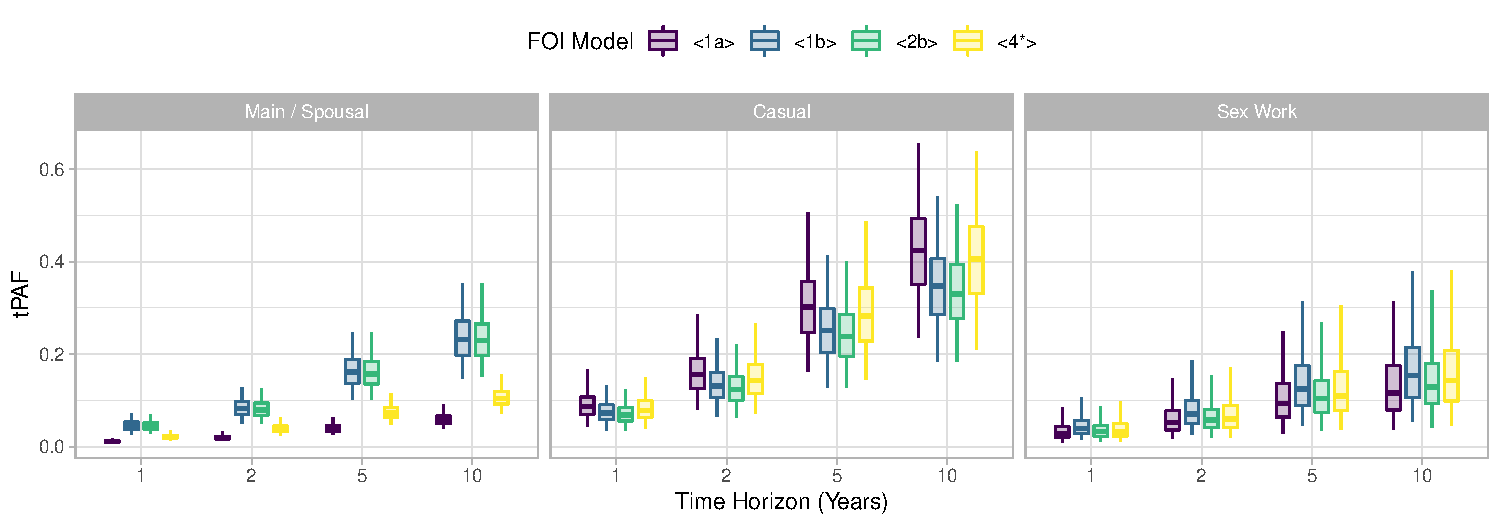
\includegraphics[width=\widefig]{foi.tpaf.3.parts}}
    \caption{Partnership types}
    \label{fig:tpaf.3.parts}
  \end{subfigure}
  \begin{subfigure}{\linewidth}
    \centerline{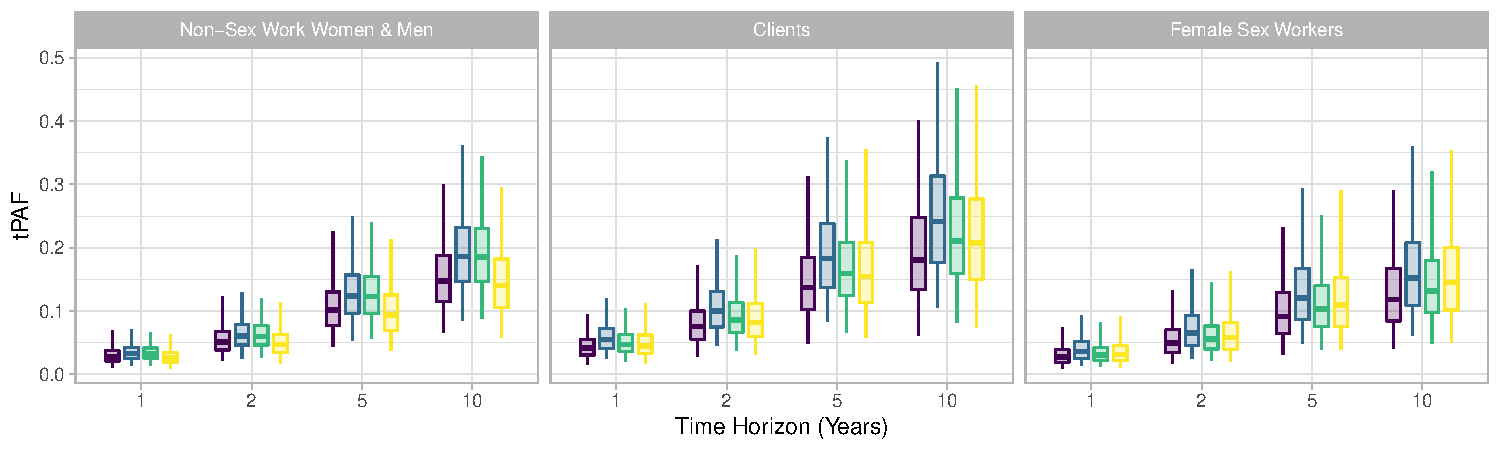
\includegraphics[width=\widefig]{foi.tpaf.3.popto}}
    \caption{Acquisition among risk groups}
    \label{fig:tpaf.3.popto}
  \end{subfigure}
  \caption{Comparison of tPAFs of different partnership types and risk groups
    under calibrated force of infection models \case{1a}, \case{1b}, \case{2b}, and \case{4*}}
  \label{fig:tpaf.3}
  \floatfoot
  tPAF: transmission population attributable fraction \cite{Mishra2014}, from $t_0 = 2000$ onward.
  FOI Model names:
  \case{1a} binomial per-partnership;
  \case{1b} binomial per-partnership-year;
  \case{2b} binomial per-year;
  \case{4*} partnership exclusion (proposed).
  Parameters were re-calibrated for each FOI model,
  and box plots reflect the median (horizontal bar),
  plus 90\% (whiskers) and 50\% (box) confidence intervals from
  the top 1000 of 100,000 model fits in each case.
\end{figure}